\documentclass{article} % For LaTeX2e
\usepackage{nips15submit_e,times}
\usepackage{hyperref}
\usepackage{url}
\usepackage{graphicx} 
\usepackage{float} 
\usepackage{subfigure} 
\usepackage{placeins}
\usepackage{float}
\usepackage{amsmath}
\usepackage{diagbox}
\usepackage{listings}
\usepackage{color}
\usepackage{amssymb}
\usepackage{pythonhighlight}
\usepackage{algorithm}
\usepackage[noend]{algpseudocode}


% \definecolor{codegreen}{rgb}{0,0.6,0}
% \definecolor{codegray}{rgb}{0.5,0.5,0.5}
% \definecolor{codepurple}{rgb}{0.58,0,0.82}
% \definecolor{backcolour}{rgb}{0.95,0.95,0.92}
 
% \lstdefinestyle{mystyle}{
%     backgroundcolor=\color{backcolour},   
%     commentstyle=\color{codegreen},
%     keywordstyle=\color{magenta},
%     numberstyle=\tiny\color{codegray},
%     stringstyle=\color{codepurple},
%     basicstyle=\footnotesize,
%     breakatwhitespace=false,         
%     breaklines=true,                 
%     captionpos=b,                    
%     keepspaces=true,                 
%     numbers=left,                    
%     numbersep=5pt,                  
%     showspaces=false,                
%     showstringspaces=false,
%     showtabs=false,                  
%     tabsize=2
% }
 
% \lstset{style=mystyle}


%\documentstyle[nips14submit_09,times,art10]{article} % For LaTeX 2.09


\title{HW2: Motion Planning}


\author{
Shuo Xu \\
Department of Computer Science and Engineering \\
\texttt{s3xu@ucsd.edu} \\
}

% The \author macro works with any number of authors. There are two commands
% used to separate the names and addresses of multiple authors: \And and \AND.
%
% Using \And between authors leaves it to \LaTeX{} to determine where to break
% the lines. Using \AND forces a linebreak at that point. So, if \LaTeX{}
% puts 3 of 4 authors names on the first line, and the last on the second
% line, try using \AND instead of \And before the third author name.

\newcommand{\fix}{\marginpar{FIX}}
\newcommand{\new}{\marginpar{NEW}}

\nipsfinalcopy % Uncomment for camera-ready version

\begin{document}


\maketitle

\begin{abstract}

\end{abstract}

\section*{Acknowledgement}
Special thanks to Ehsan Zobeid, Yu ShengDing, Yiran Xu, Zheng Liu for their hints on problem 3. 

\section{Problem 1}

\subsection{(a)}
We firstly formulate the DFS problem.

$x_t \in \mathcal{X}$ is the state at time t. $ u_{t}$ is the control at time t. $x_{t+1}=f\left(x_{t}, u_{t}\right), t=0, \ldots, T-1$ defines the state transition given control from time t to t + 1. $\ell_{t}\left(x_{t}, u_{t}\right)$ is the stage cost, and $\mathfrak{q}\left(x_{T}\right)$ is the terminal cost.

This is equivalent to a DSP problem. 
The states can be represented by a vertices set in the graph as 
$$ \mathcal{V} = (\bigcup_{t=0}^{T} \{ (t, x_t) | x_t \in \mathcal{X}\}) \cup \{\tau\}$$

The cost can be defind as 
$$\mathcal{C} :=\left\{\left(\left(t, x_{t}\right),\left(t+1, x_{t+1}\right), c\right) | c=\underset{u \in \mathcal{U}\left(x_{t}\right)}{\min } \quad \ell_{t}\left(x_{t}, u\right)\right\}\bigcup\left\{\left(\left(T, x_{T}\right), \tau, \mathfrak{q}\left(x_{T}\right)\right)\right\}$$

The optimization task can be solved by Dijkstra algorithm. Notice, the path is searched in the backward order, where we start from $\tau$ and ends at $x_0$.

\begin{algorithm}
    \caption{Dijkstra algorithm}\label{euclid}
    \begin{algorithmic}[1]
    \Procedure{Dijkstra}{start=$\tau$, end=$x_0$, distance}
    
    \State $parents \gets$ \{node : node for node in graph\}
    \State $queue \gets$all nodes in graph
    \While{$queue$ is not empty}
        \State $ prev\_node \gets$ node in queue with smallest distance to start node
        \For{each neighbour n of prev\_node}
            \State new\_dis = distance[start][prev\_node] + distance[prev\_node][n]
            \If {new\_dis $<$ distance[start][n]}
                \State $distance[start][n] \gets new\_dis$
                \State $parents[n] \gets prev\_node$
            \EndIf
        \EndFor
    \EndWhile

    \State $shortest\_path \gets [target]$
    \While{start != target}
        \State $target \gets parents[target]$
        \State $shortest\_path.append(target)$
    \EndWhile
    
    \Return {$shortest\_path$}
    
    \EndProcedure
    \end{algorithmic}
\end{algorithm}

In the worst case without early stopping, the time complexity of dynamic programming algorithm is $O(|\mathcal{V}|^3)$. 

For Dijkstra algorithm, the time complexity depends on its implementation, the simplest implementation of Dijkstra's algorithm stores the vertex set Q as an ordinary linked list or array, and extract-minimum is simply a linear search through all vertices in $queue$. In this case, the running time is $O(|E| + |\mathcal{V}|^2) = O(|\mathcal{V}|^2)$.

Thus, the Dijkstra algorithm runs more efficiently compared to DP algorithm. However, in terms of the number of investigated nodes, Dijkstra algorithm is no worse than DP algorithm with an early stopping. It saves time by avoiding investigating non-neighboured nodes at each time step.

\subsection{(b)}

Yes.

The heuristic function $h((t, x_t))$ means the lower bound on the optimal cost to get from start node $x_0$ to $x_t$.

Let's assume $h((t, x_t)) = t$. We can develop the weighted $A^*$ algorithm as
\begin{algorithm}
    \caption{$A^*$ algorithm}\label{A}
    \begin{algorithmic}[1]
    \Procedure{$A^*$}{start=$\tau$, end=$x_0$}
    
    \State $OPEN \gets \{s\}$, $CLOSED \gets \{\}, \eta \ge 1$ 
    \State $g_{s}=0, g_{i}=\infty \text { for all } i \in \mathcal{V} \backslash\{s\}$
    \While{$\tau \notin C L O S E D$}
        \State Remove $i \text { with smallest } f_{i} :=g_{i}+\epsilon h_{i}$
        \State Insert $i$ into CLOSED
        \For{$j \in \text { Children }(i) \text { and } j \notin C L O S E D$}
            \If {$g_{j}>\left(g_{i}+c_{i j}\right)$}
                \State $g_{j} \leftarrow\left(g_{i}+c_{i j}\right)$
                \State Parent $(j) \leftarrow i$
                \State Insert $j$ into OPEN
            \EndIf
        \EndFor
    \EndWhile

    \State $shortest\_path \gets [target]$
    \While{start != target}
        \State $target \gets parents[target]$
        \State $shortest\_path.append(target)$
    \EndWhile
    
    \Return {$shortest\_path$}
    
    \EndProcedure
    \end{algorithmic}
\end{algorithm}


\section{Problem 2}

\subsection{(a)}

\begin{equation*}
    \begin{aligned}
        h\left(\mathrm{x}_{\tau}\right) &= \max \left\{h^{(1)}(x_{\tau}), h^{(2)}(x_{\tau}) \right\} \\
            &= \max \left\{0, 0\right\} \\
            &= 0
    \end{aligned}
\end{equation*}

\begin{equation*}
    \begin{aligned}
        h(x_i) &=\max \left\{h^{(1)}(x_i), h^{(2)}(x_i) \right\} \\
            &\le \max \left\{ c\left(\mathbf{x}_{i}, \mathbf{x}_{j}\right)+h^{(1)} \left(\mathbf{x}_{j}\right),  c\left(\mathbf{x}_{i}, \mathbf{x}_{j}\right)+h^{(2)} \left(\mathbf{x}_{j}\right) \right\} \\
            &= c\left(\mathbf{x}_{i}, \mathbf{x}_{j}\right) + \max \left\{ h^{(1)} \left(\mathbf{x}_{j}\right), h^{(2)} \left(\mathbf{x}_{j}\right) \right\} \\
            &= c\left(\mathbf{x}_{i}, \mathbf{x}_{j}\right) + h(x_j)
    \end{aligned}
\end{equation*}

Thus $h$ is consistent.

\subsection{(b)}
\begin{equation*}
    \begin{aligned}
        h\left(\mathrm{x}_{\tau}\right) &=  h^{(1)}(x_{\tau}) + h^{(2)}(x_{\tau}) \\
            &= 0 + 0 \\
            &= 0
    \end{aligned}
\end{equation*}

\begin{equation*}
    \begin{aligned}
        h\left(\mathrm{x}_{i}\right) &= h^{(1)}\left(\mathrm{x}_{i}\right)+h^{(2)}\left(\mathrm{x}_{i}\right)\\
        &\leq c\left(\mathrm{x}_{i}, \mathrm{x}_{j}\right)+h^{(1)}\left(\mathrm{x}_{j}\right) + c\left(\mathrm{x}_{i}, \mathrm{x}_{j}\right)+h^{(2)}\left(\mathrm{x}_{j}\right) \\
        &\leq 2c\left(\mathrm{x}_{i}, \mathrm{x}_{j}\right)+h(x_j)
    \end{aligned}
\end{equation*}

Let $\epsilon = 2$. Thus $h$ is $\epsilon$ -consistent.

\subsection{(c)}
Suppose the shortest path from any node i to terminal node $\tau$ is $P_{shortest}=\{p_1=x_i, p_2, \cdots, p_m=x_{\tau}\}$.

\begin{equation*}
    \begin{aligned}
        h\left(\mathbf{x}_{i}\right) &= h\left(\mathbf{p}_{1}\right) \\
            &\leq c\left(\mathbf{p}_{1}, \mathbf{p}_{2}\right)+h\left(\mathbf{p}_{2}\right) \\
            &\leq c\left(\mathbf{p}_{1}, \mathbf{p}_{2}\right) + c\left(\mathbf{p}_{2}, \mathbf{p}_{3}\right)+h\left(\mathbf{p}_{3}\right) \\
            &\leq \sum_{i=1}^{m-1} c\left(\mathbf{p}_{i}, \mathbf{p}_{i+1}\right) + h\left(\mathbf{x}_{\tau}\right) \\
            &= \sum_{i=1}^{m-1} c\left(\mathbf{p}_{i}, \mathbf{p}_{i+1}\right) \\
            &= \textbf{dist}\left(\mathrm{x}_{i}, \mathrm{x}_{\tau}\right)
    \end{aligned}
\end{equation*}

Thus, if $h$ is consistent, then it is also admissible.


\subsection{(d)}

\begin{figure}[H]
	\centering
    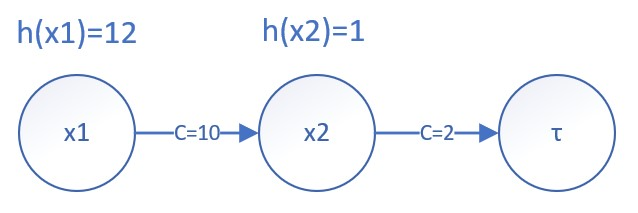
\includegraphics[width=0.6\textwidth]{images/p2_4.jpg}
    \caption{Admissible heuristic h that is not consistent}
\end{figure} 

In the graph above, It admissible because 
$h(x_1) \leq dist(x_1, \tau) = 12$ and $h(x_2) \leq dist(x_2, \tau) = 2$.

However, it's not consistent because $h(x_1) = 12 > c(x_1, x_2) + h(x_2) = 11$.

\subsection{(e)}
Let $c_{i j}>0$ for $i, j \in \mathcal{V}$ and $h$ be a consistent heuristic.
Assume all previously expanded states in CLOSED have correct g-values. Let the next state to expand be $i$ with $f_{i} :=g_{i}+h_{i} \leq f_{j}$ for all $j \in O P E N$. Suppose that $g_{i}$ is incorrect, i.e. larger than the actual least cost from s to i. Then, there must be at least one state j on an optimal path from s to i such that $j \in O P E N$ but $j \notin C L O S E D$ so that $f_{j} \geq f_{i}$. But this leads to a contradiction:

$$f_{i}=g_{i}+h_{i}>V_{s, i}^{*}+h_{i}=g_{j}+V_{j i}^{*}+h_{i} \geq  g_{j}+h_{j}=f_{j}$$

So if the heuristic function used in $A^{*}$ is consistent, then $A^{*}$ will not re-open nodes.

\subsection{(f)}
It's not consistent not admissible.

\textbf{Proof}

Suppose $x_1 = 0.001, x_2 = -1, x_{\tau} = 0$.

Then $$h(x_1) = 0.001 + 0.4 \times 0.001 = 0.0014, $$ $$h(x_2) = -1 - 0.4 \times 1 = -1.4, $$ $$c(x_1, x_2) = (0.001 + 1)^2 = 1.002001$$

Thus, 
$$h(x_1) = 0.0014 \ge h(x_2) + c(x_1, x_2) = -0.397999$$

So the heuristic function is not consistent.

Since
$$ h(x_1) = 0.0014 > dist(x_1, x_{\tau}) = 0.001, $$
the heuristic function is also not admissible.


\section{Problem 3}
\subsection{(a)}

The problem can be formulated as following.

Suppose the cell phone's battery $x$ can take on the value from $\mathcal{X}={1,2,\dots, n}$. The choice of whether to charge or not given current state is denoted as $\pi(x) \in \mathcal{U} = \{0, 1\}$, where 1 means recharge and 0 means not.

The transition model is defined as below. 
$$p_{f}\left(x_{t+1} | x_{t}, \pi\left(x_{t}\right)\right)=
\begin{cases}
q& x_{t+1}=1, \pi(x_t)=1\\
1 - q & x_{t+1}=x_t, \pi(x_t)=1 \\
P(i, j) & x_t = i, x_{t+1}=j, \pi(x_t)=0 \\
0 & else
\end{cases}$$
where $P(i, j)$ describes the probability of transitioning from state i to state j.

The stage cost is defined as 
\begin{equation*}
    \begin{aligned}
        \ell (x_t, \pi(x_t)) &= \pi(x_t)[qc + (1-q)\times0] + (1-\pi(x_t))[-\sum_{x_{t+1}}P(x_t, x_{t+1})r(x_t)] \\
                &= \pi(x_t)qc - (1-\pi(x_t))\sum_{x_{t+1}}P(x_t, x_{t+1})r(x_t) \\
                &= \pi(x_t)qc - (1-\pi(x_t))r(x_t)\sum_{x_{t+1}}P(x_t, x_{t+1}) \\
                &= \pi(x_t)qc - (1-\pi(x_t))r(x_t)
    \end{aligned}
\end{equation*}

The discounting problem is formulated as

$$V^{*}(x)=\min _{\pi} V^{\pi}(x) :=\mathbb{E}\left[\sum_{t=0}^{\infty} \gamma^{t} \ell\left(x_{t}, \pi\left(x_{t}\right)\right) | x_{0}=x\right]$$
$$s.t. \quad x_{t+1} \sim p_{f}\left(\cdot | x_{t}, \pi\left(x_{t}\right)\right)$$
$$x_{t} \in \mathcal{X}$$
$$\pi\left(x_{t}\right) \in \mathcal{U}$$


Substitute the stage cost and transition model into the discounting equation into the Bellman equation, we have
% \begin{equation*}
%     \begin{aligned}
%         V^{*}(x) &= \min _{u \in \mathcal{U}(x)}\left(\ell(x, u)+\gamma \sum_{x^{\prime} \in \mathcal{X}} p_{f}\left(x^{\prime} | x, u\right) V^{*}\left(x^{\prime}\right)\right) \\
%                  &= \min _{u \in \mathcal{U}(x)} \{ uqc - (1-u)r(x) + u\gamma[qV^*(1) + (1-q)V^*(x)] + (1-u)\gamma \sum_{x'\in\mathcal{X}}[P(x, x')V^*(x')]\} \\
%                  &= \min _{u \in \mathcal{U}(x)} \{ u[qc + \gamma(qV^*(1) + (1-q)V^*(x))] + (1-u)[-r(x) + \gamma \sum_{x'\in\mathcal{X}}P(x, x')V^*(x')]\} \\
%     \end{aligned}
% \end{equation*}

$$ V^{*}(x) = \min _{u \in \mathcal{U}(x)} 
\begin{cases}
    qc + \gamma(qV^*(1) + (1-q)V^*(x)) & u=1\\
    -r(x) + \gamma \sum_{x'\in\mathcal{X}}P(x, x')V^*(x') & u=0 \\
\end{cases}
$$

\subsection{(b)}

The claim can be proved using induction. I will try to prove that in value iteration, $V_{t+1}$ is increasing if $V_t$ is increasing.

Since value iteration will get the optimal value which is irrelavant to the initalization of $V_0(x)$, we can assign specific numbers to $V_0(i)$ that is increasing in i.

Suppose we have all the $V_t(i)$ that is increasing in i, then we will prove $V_{t+1}(i)$ is also increasing in i. According to the value iteration algorithm, we have

$$V_{t+1}(x) =
\begin{cases}
    -r(x) + \gamma \sum_{x'\in\mathcal{X}}P(x, x')V_t(x') & u=0 \\
    qc + \gamma [qV_t(1) + (1-q)V_t(x)] & u=1 \\
\end{cases}$$

If $a < b$ and $c < d$, it's guaranteed that $min(a,b) < min(c,d)$, so we only need to prove that $Q_t(i, 0) \ge Q_t(i-1, 0)$ and $Q_t(i, 1) < Q_t(i - 1, 1)$, then we will get $V_t(i) \ge V_t(i - 1)$ because $V_t(i) = min[Q_t(i, 0), Q_t(i, 1)]$.

$$V_{t+1}(x)=\min _{u \in \mathcal{U}(x)}\left[\ell(x, u)+\gamma \sum_{x^{\prime} \in \mathcal{X}} p_{f}\left(x^{\prime} | x, u\right) V_{t}\left(x^{\prime}\right)\right], \quad \forall x \in \mathcal{X}$$. This means we only need to prove that $V_{t+1}(x)$ is increasing when $u=0$ and $u=1$, separately.

When $u=1$, since $(1-q) \ge 0$, $\gamma > 0$ and $V_t(x)$ is increasing, $V_{t+1}(x)$ is also monotonously not decreasing.

When $u=0$, we have
\begin{equation*}
    \begin{aligned}
		V_{t+1}(x) &= -r(x)+\gamma \sum_{x^{\prime} \in \mathcal{X}} P\left(x, x^{\prime}\right) V_{t}\left(x^{\prime}\right) \\
    \end{aligned}
\end{equation*}
Since $-r(x)$ is increasing in i, we only need to prove $\sum_{x^{\prime} \in \mathcal{X}} P\left(x, x^{\prime}\right) V_{t}\left(x^{\prime}\right)$ is also increasing. We abbreviated $P\left(x, x^{\prime}\right)$ as $P_{x, x^{\prime}}$ 

\begin{equation*}
    \begin{aligned}
		\sum_{x^{\prime} \in \mathcal{X}} P_{x, x^{\prime}} V_{t}\left(x^{\prime}\right) &= \left(\sum_{x^{\prime}=1}^{n} P_{x x^{\prime}}\right) V_t(1)+\sum_{x^{\prime}=2}^{n}\left(\sum_{l=x^{\prime}}^{n} P_{x l}\right)\left(V_t(x^{\prime})-V_t(x^{\prime}-1)\right) \\
    \end{aligned}
\end{equation*}

Since $V_t(x^{\prime})-V_t(x^{\prime}-1) > 0$, and $\sum_{l=x^{\prime}}^{n} P_{x l}$ is increasing in x, it's obvious $\sum_{x^{\prime}=2}^{n}\left(\sum_{l=x^{\prime}}^{n} P_{x l}\right)\left(V_{t}\left(x^{\prime}\right)-V_{t}\left(x^{\prime}-1\right)\right)$ also increase in i. So $\sum_{x^{\prime} \in \mathcal{X}} P_{x, x^{\prime}} V_{t}\left(x^{\prime}\right)$ is increasing in $x$.

Thus, we've proved $V_{t+1}(x)$ is also increasing in i.

By induction, we've proved that $V_{t}(x)$ is increasing in i.

\subsection{(c)}

According to 
$$V^{*}(x)=\min _{u \in \mathcal{U}(x)} \left\{\begin{array}{ll}{q c+\gamma\left(q V^{*}(1)+(1-q) V^{*}(x)\right)} & {u=1} \\ {-r(x)+\gamma \sum_{x^{\prime} \in \mathcal{X}} P\left(x, x^{\prime}\right) V^{*}\left(x^{\prime}\right)} & {u=0}\end{array}\right.$$
we noticed that when $u=1$, $V^*(x) = q c+\gamma\left(q V^{*}(1)+(1-q) V^{*}(x)\right)$, thus $$V^*(x) = \frac{1}{1 - \gamma + \gamma q} (q c + \gamma q v^*(1))$$ which is a constant irrelevant with $x$. 

Thus we have $$Q^*(x, u) = 
\begin{cases}
    -r(x)+\gamma \sum_{x^{\prime} \in \mathcal{X}} P\left(x, x^{\prime}\right) V^{*}\left(x^{\prime}\right) & u=0\\
    \frac{1}{1 - \gamma + \gamma q} (q c + \gamma q v^*(1)) & x_{t+1}=x_t, \pi(x_t)=1 \\
\end{cases}$$

Thus, 

\begin{equation*}
    \begin{aligned}
        \Delta_x & = Q^*(x, 0) - Q^*(x, 1) \\
        &= -r(x)+\gamma \sum_{x^{\prime} \in \mathcal{X}} P\left(x, x^{\prime}\right) V^{*}\left(x^{\prime}\right) - {1 - \gamma + \gamma q} (q c + \gamma q v^*(1))
    \end{aligned}
\end{equation*}

In the last section, we've already proved that $-r(x)+\gamma \sum_{x^{\prime} \in \mathcal{X}} P\left(x, x^{\prime}\right) V^{*}\left(x^{\prime}\right)$ is an  increasing function, and since the rest of the difference above is constant, $\Delta_x$ is also a increasing function.

Thus, $\Delta_x$ would have at most one zero point. Suppose the zero point is $t$, when $x < t, Q^*(x, 0) \le Q^*(x, 1)$, and when $x > t, Q^*(x, 0) \ge Q^*(x, 1)$. Thus it's proved to be threshold. If the zero point does not exist, we can simply incorporate this case as $t=-\infty$ if $u=0$ and $t=\infty$ if $u=1$.

\section{Problem 4}

\subsection{Introduction}
The objective of this planning problem is to find a feasible (and cost-efficient) path in a 3D space with box obstacles from the current configuration of the robot to its goal configuration. 

The robot is defined as a point without volume. The cost is chosen from distance functions, like euclidean distance, infinite norm, Manhattan distance, etc.

To guide the robot from start point to the goal, I implemented 2 search algorithms based on different strategies: search-based RTAA* and sample based Bi-directional RRT.

\subsection{Problem Formulation}
Firstly, we define a cuboid set as $Cub = \{ min, max | min, max \in R^3, min \le max\}$, where $min \le max$ means the coordinate of min on all axis is smaller than that of max.
\begin{itemize}
    \item 3D space: $\mathcal{S} \subseteq R^3$.
    \item Boundary: a cuboid $\mathcal{B} \in Cub$.
    \item Obstacles: $\mathcal{O} \subseteq Cub$, since all the obstacles in the space are box-shaped.
    \item Start point, goal point: $start, goal \in R^3$.
\end{itemize}

We discretize $\mathcal{S}$ into discrete points denoted as $\mathcal{G} \subset \mathcal{S}$. The original planning task is converted into a shortest path problem, which is defined as below.

\begin{itemize}
    \item Node: $\mathcal{V} = \{v | v \in \mathcal{G}, v \notin \mathcal{O}\}$.
    \item Start node: $s \in \mathcal{V}$.
    \item Goal node: $\tau \in \mathcal{V}$.
    \item Cost:	$$C(v_i, v_{i+1})=
    \begin{cases}
    ||v_i - v_{i+1}||_2 & \text{if $v_i$ and $v_{i+1}$ are neighboured} \\
    \infty & \text{else} \\
    \end{cases}$$
    \item Path: an ordered list $Q :=\left(v_{1}, v_{2}, \ldots, v_{q}\right)$ of nodes $v_{k} \in \mathcal{V}$.
    \item Set of all paths from $s \in \mathcal{V}$ to $\tau \in \mathcal{V} : \mathbb{Q}_{s, \tau}$.
    \item Path Length: sum of the arc lengths over the path: $J^{Q}=\sum_{t=1}^{q-1} c_{t, t+1}$.
\end{itemize}

The objective is to find a path $Q^{*}=\underset{Q \in \mathbb{Q}_{s, \tau}}{\arg \min } J^{Q}$ that has the smallest length from node $s \in \mathcal{V}$ to node $\tau \in \mathcal{V}$.

\subsection{Technical Approach}

One difference between search-based algorithm and sample-based algorithm is in the discretization approach. In the search-based case, the grid is aligned with axis, the neighboured nodes are defined as the immediate-neighboured grid points and the immediate-neighboured diagonal points, because we support both straight move and diagonal move. In the sampling-based algorithm, the nodes are no more constrained to be grid points, but randomly sampled in the valid configuation space.

\subsubsection{RTAA*}

The time complexity of A* depends on the heuristic. In the worst case of an unbounded search space, the number of nodes expanded is exponential in the depth of the solution (the shortest path) d: O(bd), where b is the branching factor (the average number of successors per state). RTAA* guarantees that the goal is reached in a finite number of steps.

$\mathrm{A}^{*}$ is complete and will always find a solution if one exists provided $d(x, y)>\varepsilon>0$ for fixed $\varepsilon$. The most admissible and consistent heuristics. RTAA* guarantee admissible and consistent heuristics. And the heuristics is monotonically increasing.

A* is also optimally efficient for any heuristic h, meaning that no optimal algorithm employing the same heuristic will expand fewer nodes than A*, except when there are multiple partial solutions where h exactly predicts the cost of the optimal path. 

The RTAA* algorithm\ref{RTAA} is based on the A* algorithm. The main idea is that the adaptive A* makes the heuristics more informed after each A* search in order to speed up future A* searches. Compared to original A*, which may perform myopically at local minima, RTAA* \textbf{updates the heuristic over time by repeatedly move to the most promising adjacent cell using and updating a heuristic}. The heuristic updates make h more informed while ensuring it remains admissible and consistent.

Moreover, the robot is guaranteed to reach the goal in a finite number of steps if 
\begin{itemize}
    \item All edge costs are bounded from below: $c_{i j} \geq \Delta>0$
    \item The graph is finite size and there exists a finite-cost path to the goal
    \item All actions are reversible ensures that we do not get stuck in a local min
\end{itemize}

We now formulate the main idea behind Adaptive A*.
Here we define some variables that will appear in the peudocode. Notice that the Variables annotated with [A*] are updated during the call to astar() (= line 4 in the pseudo code), which performs a (forward) A* search guided by the current heuristics from the current state of the agent toward the goal states until a goal state is about to be expanded or $lookahead > 0$ states have been expanded.

\textbf{constants and functions}
\begin{itemize}
    \item S: set of states of the search task, a set of states
    \item GOAL: set of goal states, a set of states
    \item A(): sets of actions, a set of actions for every state
    \item succ(): successor function, a state for every state-action pair
    \item lookahead: number of states to expand at most, an integer larger than zero
    \item movements: number of actions to execute at most, an integer larger than zero
    \item scurr: current state of the agent, a state [USER]
    \item c: current action costs, a float for every state-action pair [USER]
    \item h: current (consistent) heuristics, a float for every state [USER]
    \item g: g-values, a float for every state [A*]
    \item CLOSED: closed list of A* (= all expanded states), a set of states [A*]
    \item $\bar{s}$: state that A* was about to expand when it terminated, a state [A*]
\end{itemize}

\begin{algorithm}[H]
    \caption{$RTAA^*$ algorithm}\label{RTAA}
    \begin{algorithmic}[1]
    \Procedure{$RTAA^*$}{start=$x_0$, end=$\tau$}
    
    \While{$s_{\mathrm{curr}} \notin G O A L$}
        \State lookahead $:=$ any desired integer greater than zero
        \State astar()
        \If {$\overline{s}=F A I L U R E$}
            \Return {$F A I L U R E$}
        \EndIf
        \For{all $s \in C L O S E D$}
            \State $h[s] :=g[\overline{s}]+h[\overline{s}]-g[s]$
        \EndFor
        \State movements $:=$ any desired integer greater than zero
        \While{$S_{\mathrm{curr}} \neq \overline{S}$ AND movements $>0$}
            \State $a :=$ the action in $A\left(s_{\text { curr }}\right)$ on the cost-minimal trajectory from $s_{\text { curr }}$ to $\overline{s}$
            \State $s_{\mathrm{curr}} :=\operatorname{succ}\left(s_{\mathrm{curr}}, a\right)$
            \State movements $:=$ movements $-1$
        \EndWhile
        \EndWhile
    \Return {$S U C C E S S$}    
    \EndProcedure
    \end{algorithmic}
\end{algorithm}

\subsubsection{Bi-directional RRT}

The main idea of Bi-directional RRT is that a tree is constructed from random samples with root xs. The tree is grown until it contains a path to $x_{\tau}$. RRTs are well-suited for
single-shot planning between a single pair of $x_s$ and $x_{\tau}$ (single query). Bi-direction RRT expand two trees at the same time, which can accelerate the search of the tree. 


RRT and RRT-Connect are probabilistically complete, which means the probability that a feasible path will be found if one exists, approaches 1 exponentially as the number of samples approaches infinity.

But RRT is not optimal. The probability that RRT converges to an optimal
solution, as the number of samples approaches innity, is zero under
reasonable technical assumptions.


\begin{algorithm}[H]
    \caption{$Bi-directional RRT^*$ algorithm}\label{RRT}
    \begin{algorithmic}[1]
    \Procedure{$Bi_RRT^*$}{start=$x_0$, end=$\tau$}
    
    \While{$s_{\mathrm{curr}} \notin G O A L$}
        \State $V_{a} \leftarrow\left\{x_{s}\right\} ; E_{a} \leftarrow \emptyset ; V_{b} \leftarrow\left\{x_{\tau}\right\} ; E_{b} \leftarrow \emptyset$
        \For{$i=1 \ldots n$}
            \State $X_{\text {rand}} \leftarrow$ SAMPLEFREE $( )$
            \State $x_{\text { nearest }} \leftarrow \mathrm{NEAREST}\left(\left(V_{a}, E_{a}\right), x_{\text {rand}}\right)$
            \State $x_{c} \leftarrow$ STEER $\left(x_{\text {nearest}}, x_{\text {rand}}\right)$

            \If {$x_{c} \neq x_{\text {nearest}}$}
                \State $V_{a} \leftarrow V_{a} \cup\left\{x_{c}\right\} ; E_{a} \leftarrow\left\{\left(x_{n e a r e s t}, x_{C}\right),\left(x_{c}, x_{n e a r e s t}\right)\right\}$ 
                \State $x_{\text {nearest}}^{\prime} \leftarrow \mathrm{N}$ EAREST $\left(\left(V_{b}, E_{b}\right), x_{c}\right)$
                \State $x_{c}^{\prime} \leftarrow \operatorname{STEER}\left(x_{\text {nearest}}^{\prime}, x_{C}\right)$
                \If {$x_{c}^{\prime} \neq x_{\text {nearest}}^{\prime}$}
                    $V_{b} \leftarrow V_{b} \cup\left\{x_{c}^{\prime}\right\} ; E_{b} \leftarrow\left\{\left(x_{n e a r e s t}^{\prime}, x_{c}^{\prime}\right),\left(x_{c}^{\prime}, x_{n e a r e s t}^{\prime}\right)\right\}$
                \EndIf 
            \If {$x_{c}^{\prime}=x_{c}$}
                \State \textbf{Return} \text{SOLUTION}
            \EndIf

            \If {$\left|V_{b}\right|<\left|V_{a}\right|$}
                \State $Swap\left(\left(V_{a}, E_{a}\right),\left(V_{b}, E_{b}\right)\right)$
            \EndIf            
            \EndIf
        \EndFor
    \EndWhile
    \EndProcedure
    \end{algorithmic}
\end{algorithm}


\subsection{Results}

Here, we compare the performance of RRT and A*.

\textbf{RRT}
\begin{itemize}
    \item Sparse exploration requires little memory and computation
    \item Solutions can be highly sub-optimal and require post-processing (path smoothing) which may be difficult
\end{itemize}

\textbf{Weighted A*}
\begin{itemize}
    \item Systematic exploration may require a lot of memory and computation
    \item Returns a path with (sub-)optimality guarantees
\end{itemize}

In the table, we observed that 
\begin{itemize}
    \item Bi-directional RRT usually generates shorter path than RTAA*.
    \item Bi-directional RRT is not good at Monza and Maze, because the points are enclosed in mostly surrounded space with only a little exit on the wall. But RTAA* handles the case better.
\end{itemize}

In the RTAA* implementation, I used dynamically adjusted step size. The step size is large at first and when it approaches the goal, the step size will become smaller. In practice, this do accelerate the searching process.

In terms of the smoothness of the path generated by two algorithms, RTAA* is much more straight, while RRT is more zigzaging. This may be improved by performing smoothing techniques.

In term of the search efficiency, RRT is less efficient by searching lots of useless space. While RTAA* with proper heuristic function could generated a path that has a tendency towards the goal. 

I also tried out a few different heuristics, and the conclusion is that under most case, the euclidean distance performs well. But in the flappy bird and Monza have better performance when using infinite distance.


\begin{table}[H]
    \centering
    \caption{Performance comparison}
\begin{tabular}{|c|*{3}{c|}}
    \hline
    Algorithm + scene & path length & number of moves & planning time \\
    \hline
    Bi-RRT + single cube & 7.346 & 13 & 4 \\
    \hline
    Bi-RRT + flappy bird & 34.967 & 57 & 52 \\
    \hline
    Bi-RRT + tower & 39.04 & 64 & 172\\
    \hline
    Bi-RRT + room & 13.127 & 22 & 12 \\
    \hline
    Bi-RRT + window & 33.812 & 55 & 16 \\
    \hline
    Bi-RRT + monza & 75.813 & 124 & 2241 \\
    \hline
    Bi-RRT + maze & 112.303 & 179 & 2565 \\
    \hline
    RTAA* + single cube & 1.37 & 49 & 0 \\
    \hline
    RTAA* + flappy bird & 9.92 & 685 & 0 \\
    \hline
    RTAA* + tower & 18.33 & 1042 & 0 \\
    \hline
    RTAA* + room & 9.66 & 546 & 0 \\
    \hline
    RTAA* + window & 5.09 & 375 & 0 \\
    \hline
    RTAA* + monza & 162.74 & 367 & 0 \\
    \hline
    RTAA* + maze & 344.24 & 1118 & 0 \\
    \hline
\end{tabular}
\end{table}

Here are screen shots of visualized path. Notice, the red line in the RTAA* figures are the real time trajectory, while ones in the RRT figures are the RRT trees, only the blue lines are the trajectory of robots.

\subsection{RTAA*}

\begin{figure}[H]
	\centering
    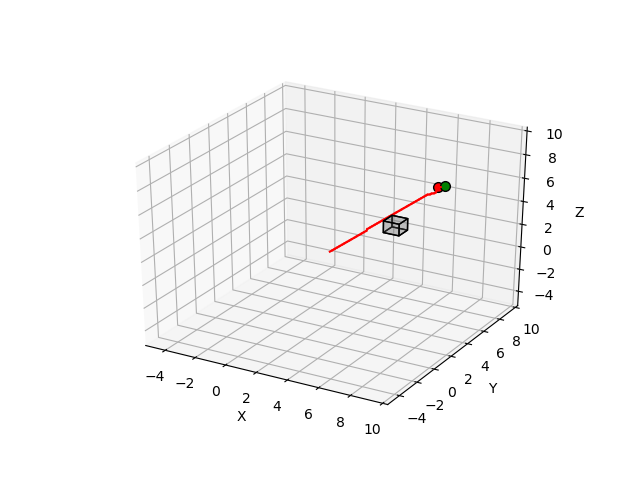
\includegraphics[width=0.7\textwidth]{./images/RTAA-singlecube.png}
    \caption{RTAA-singlecube}
    \label{RTAA-singlecube}
\end{figure}

\begin{figure}[H]
	\centering
    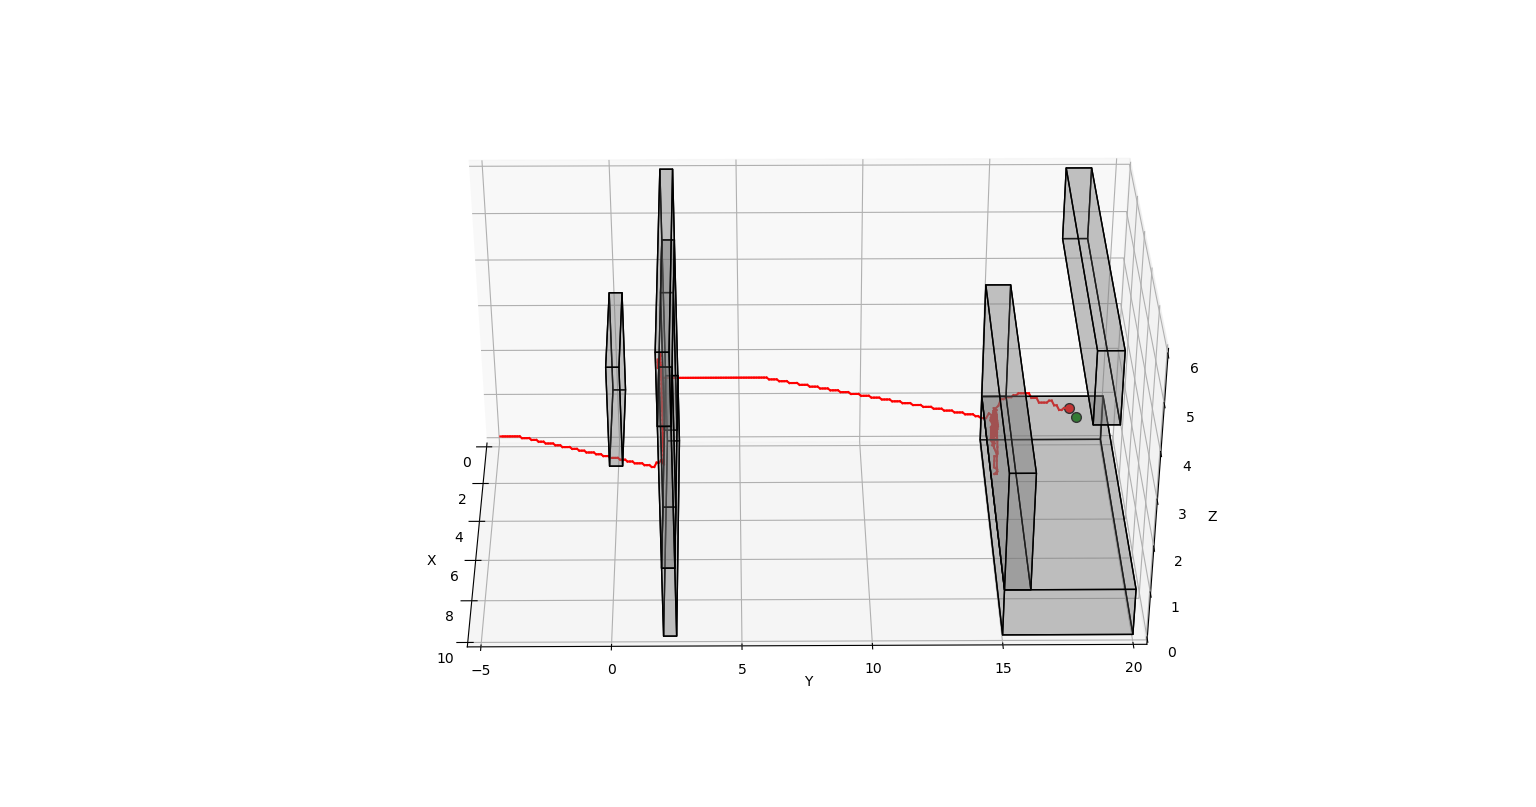
\includegraphics[width=0.7\textwidth]{./images/RTAA-window.png}
    \caption{RTAA-window}
    \label{RTAA-window}
\end{figure}

\begin{figure}[H]
	\centering
    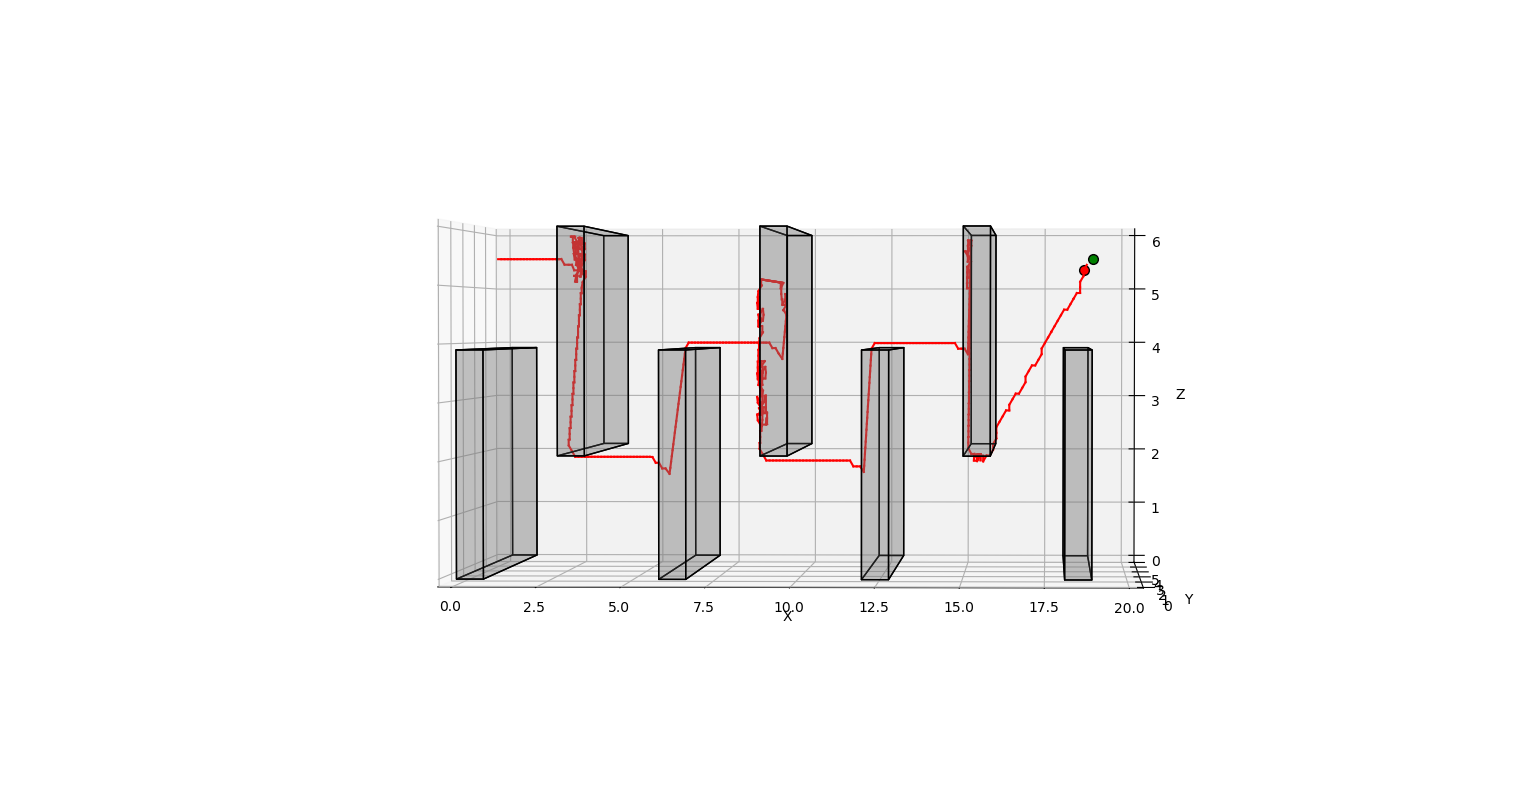
\includegraphics[width=0.7\textwidth]{./images/RTAA-flappybird.png}
    \caption{RTAA-flappy}
    \label{RTAA-flappy}
\end{figure}

\begin{figure}[H]
	\centering
    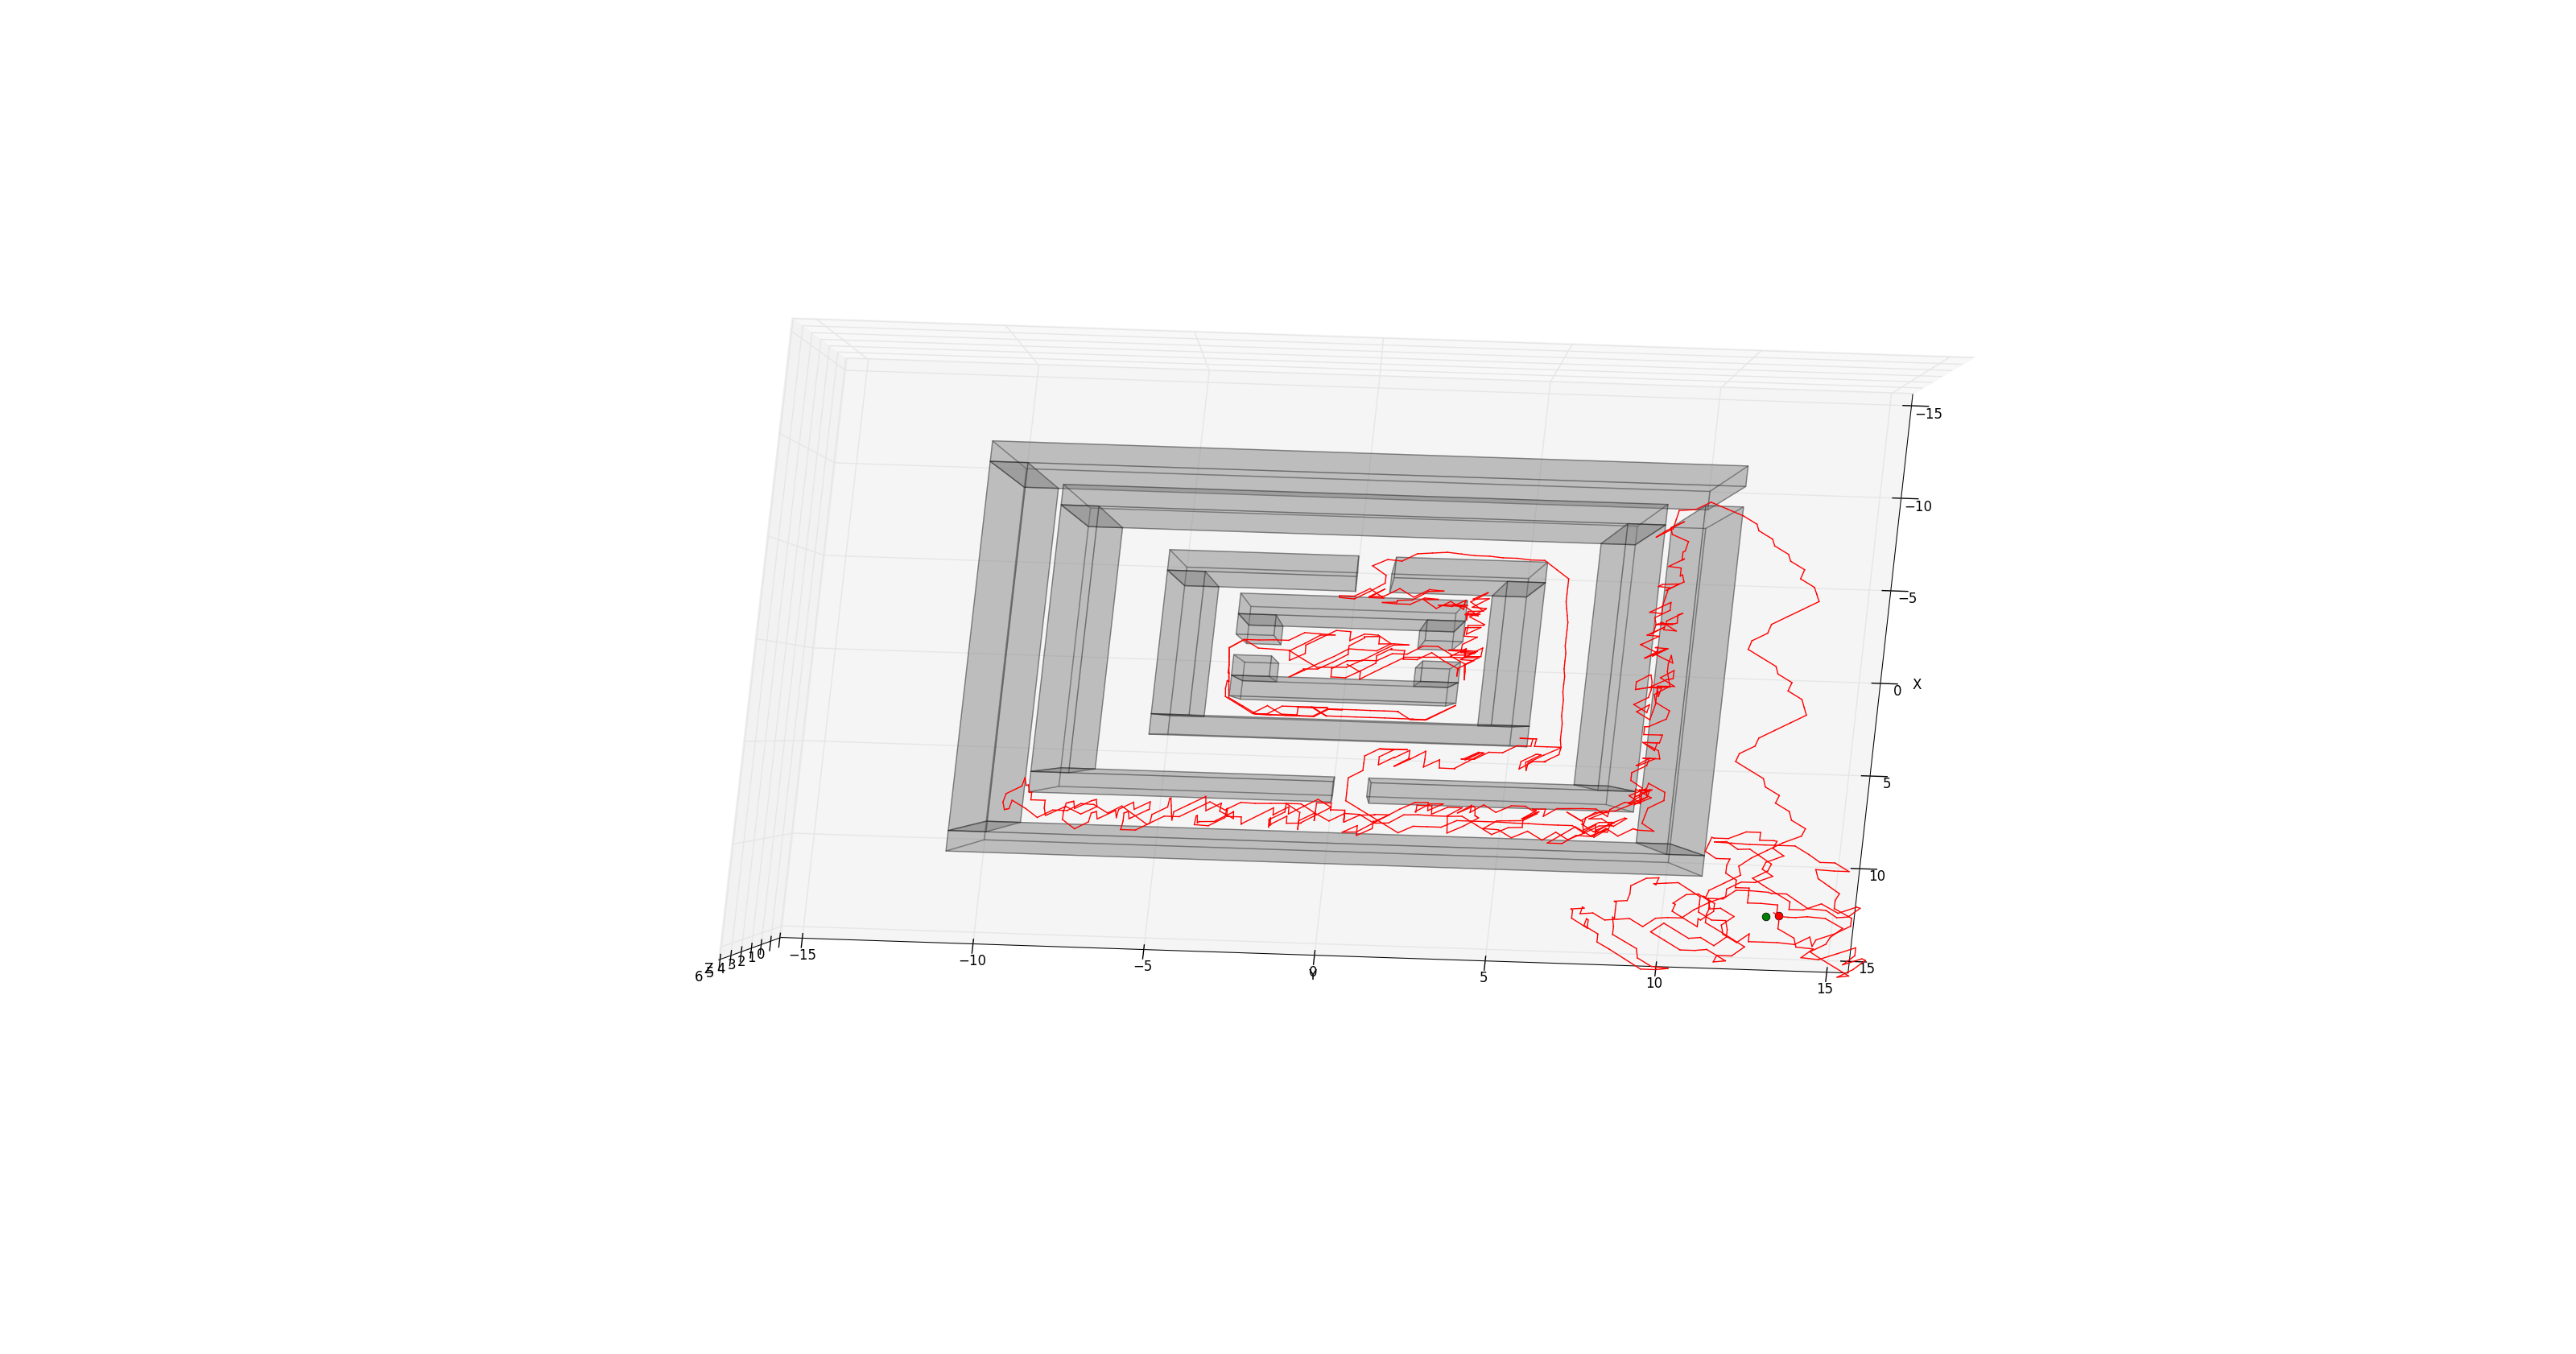
\includegraphics[width=0.7\textwidth]{./images/RTAA-maze.png}
    \caption{RTAA-maze}
    \label{RTAA-maze}
\end{figure}

\begin{figure}[H]
	\centering
    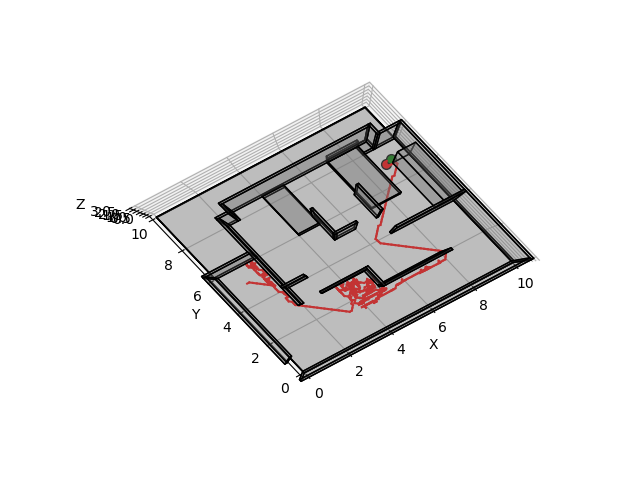
\includegraphics[width=0.7\textwidth]{./images/RTAA-room.png}
    \caption{RTAA-room}
    \label{RTAA-room}
\end{figure}

\begin{figure}[H]
	\centering
    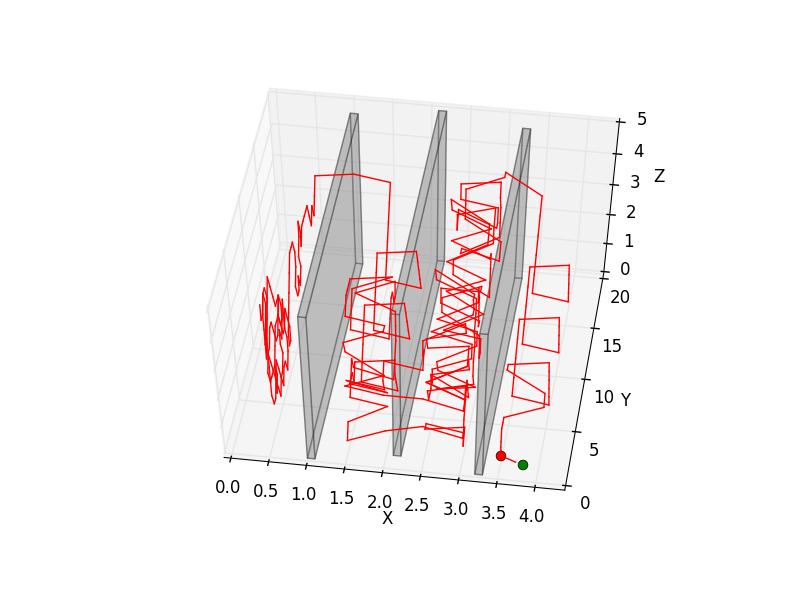
\includegraphics[width=0.7\textwidth]{./images/RTAA-monza.png}
    \caption{RTAA-monza}
    \label{RTAA-monza}
\end{figure}

\begin{figure}[H]
	\centering
    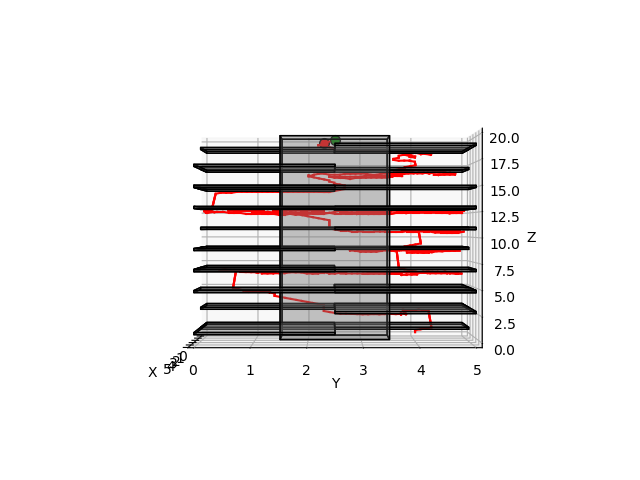
\includegraphics[width=0.7\textwidth]{./images/RTAA-tower.png}
    \caption{RTAA-tower}
    \label{RTAA-tower}
\end{figure}

\subsection{Bi-Directional RRT}

\begin{figure}[H]
	\centering
    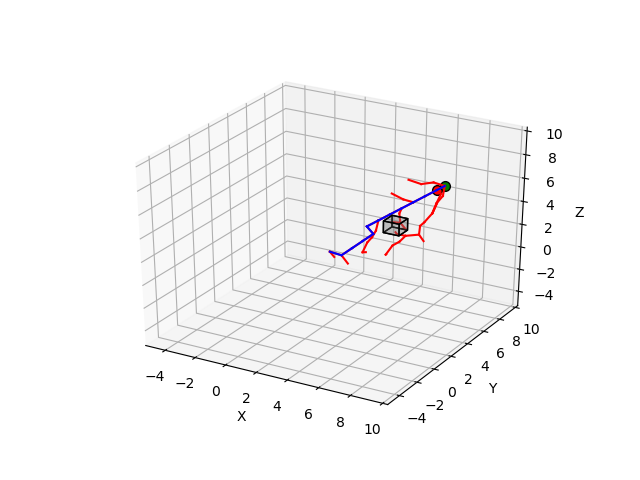
\includegraphics[width=0.7\textwidth]{./images/RRT-singlecube.png}
    \caption{RRT-singlecube}
    \label{RRT-singlecube}
\end{figure}

\begin{figure}[H]
	\centering
    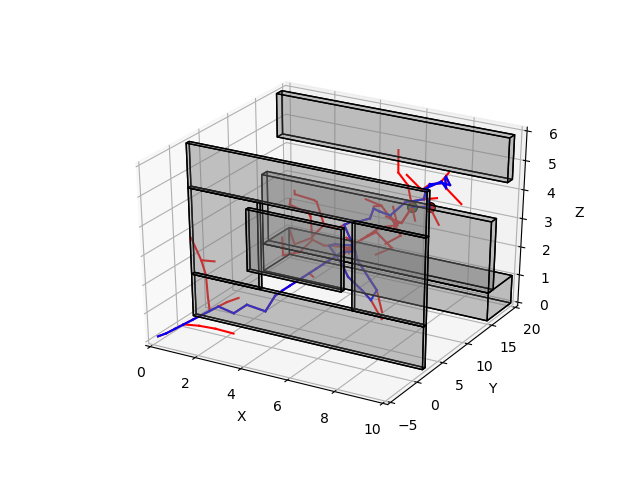
\includegraphics[width=0.7\textwidth]{./images/RRT-window.png}
    \caption{RRT-window}
    \label{RRT-window}
\end{figure}

\begin{figure}[H]
	\centering
    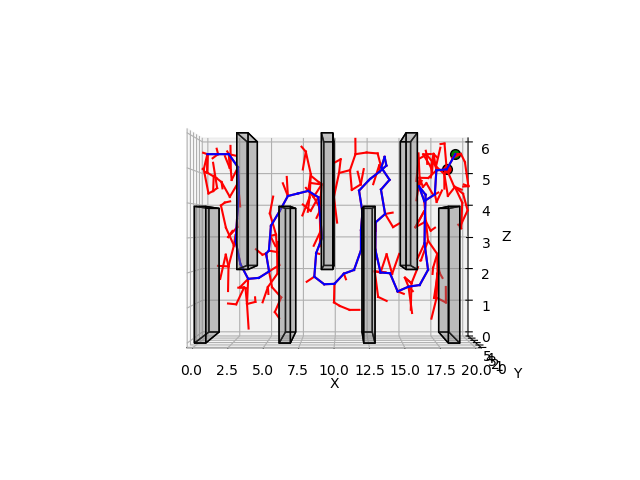
\includegraphics[width=0.7\textwidth]{./images/RRT-flappybird.png}
    \caption{RRT-flappy}
    \label{RRT-flappy}
\end{figure}

\begin{figure}[H]
	\centering
    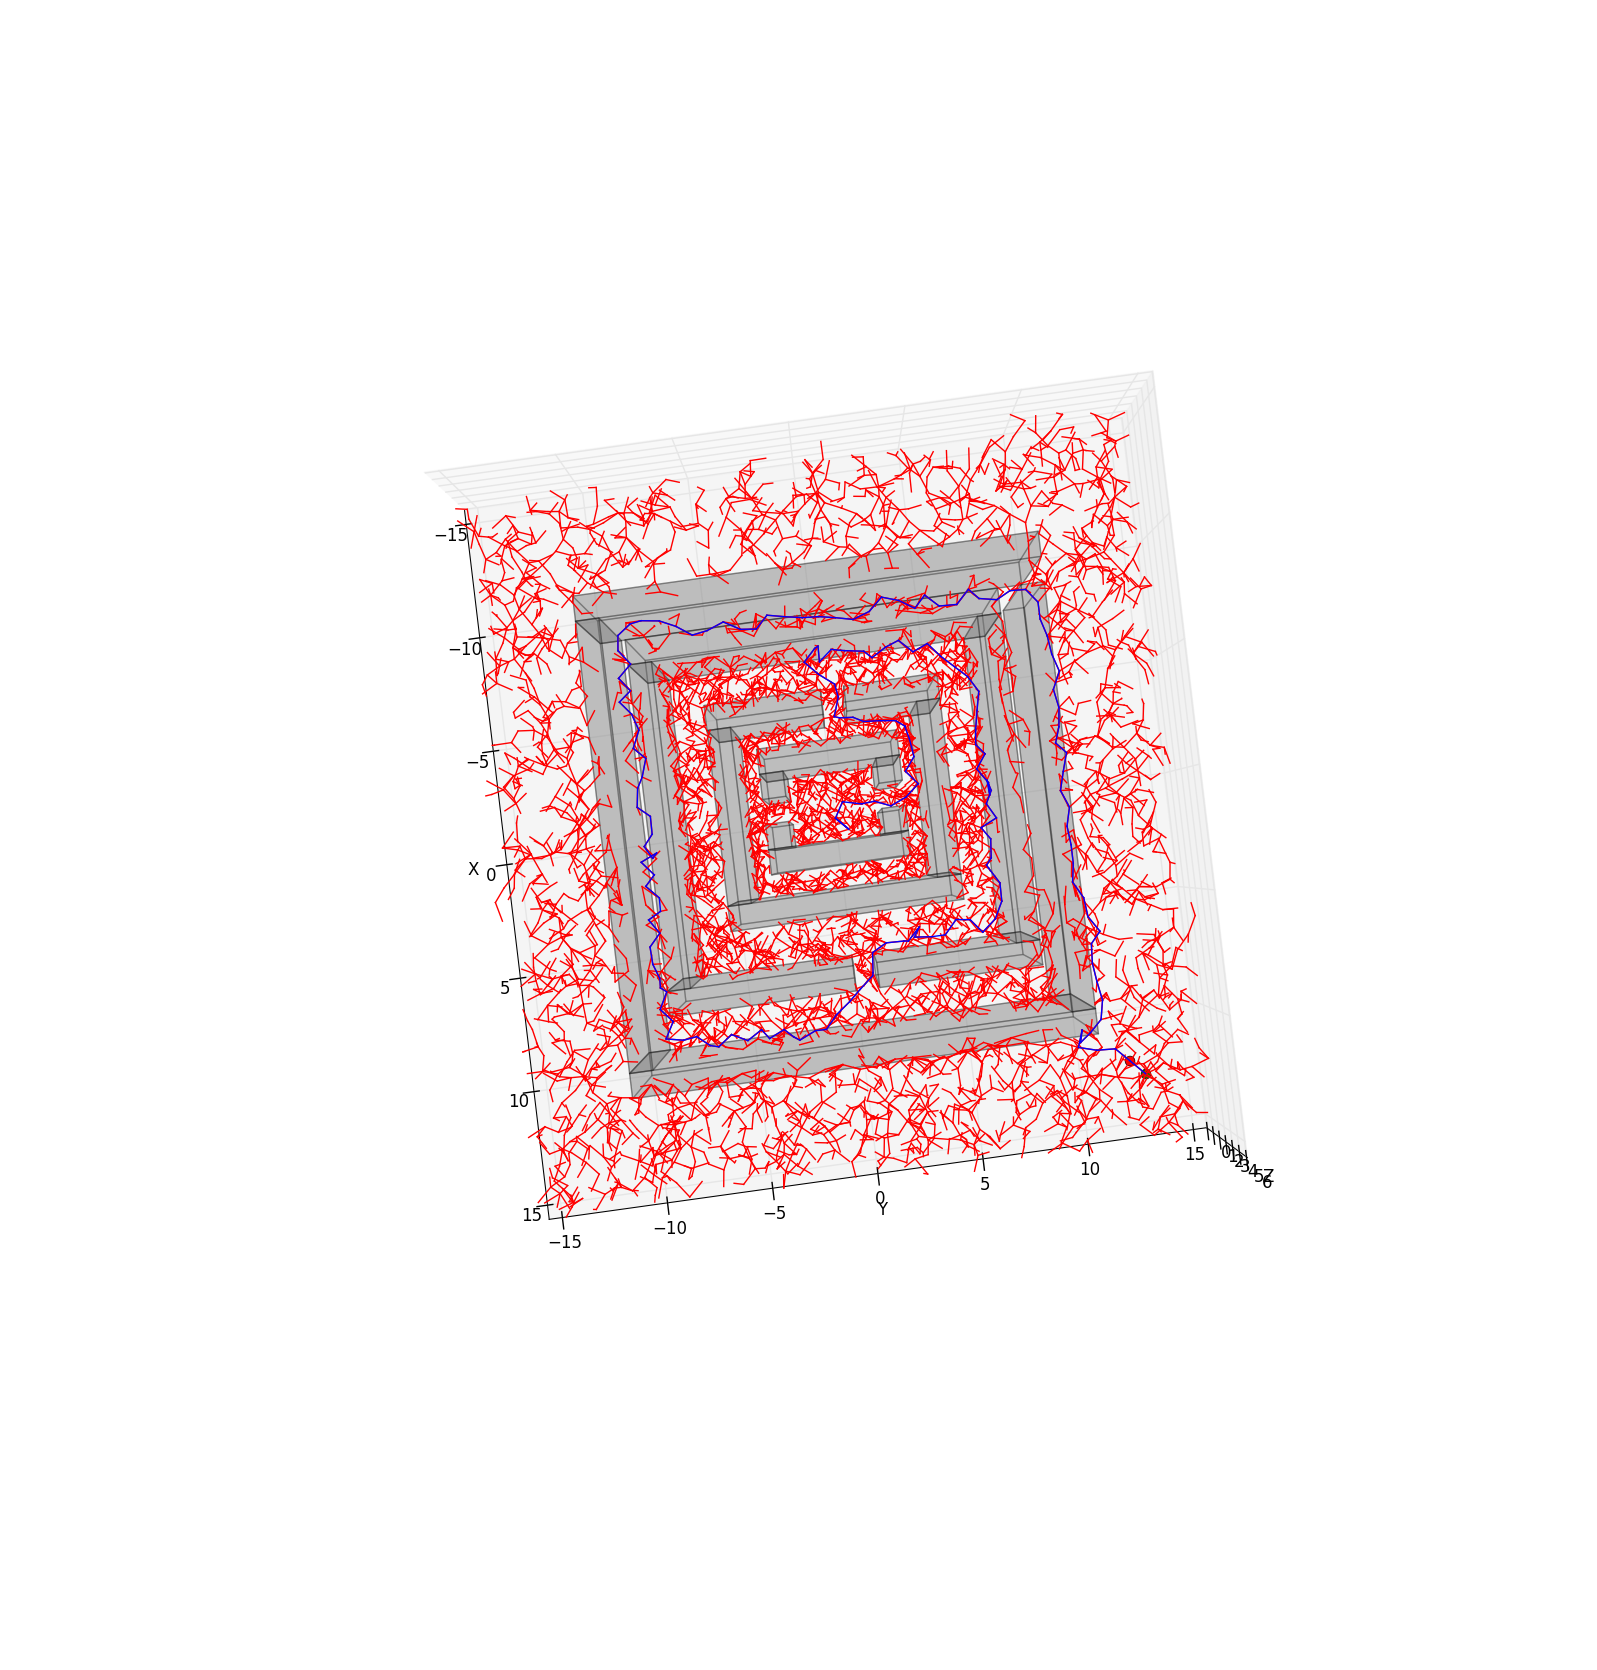
\includegraphics[width=0.7\textwidth]{./images/RRT-maze.png}
    \caption{RRT-maze}
    \label{RRT-maze}
\end{figure}

\begin{figure}[H]
	\centering
    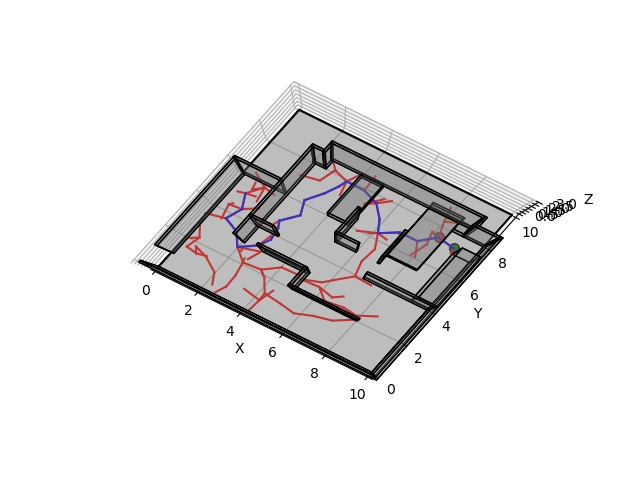
\includegraphics[width=0.7\textwidth]{./images/RRT-room.png}
    \caption{RRT-room}
    \label{RRT-room}
\end{figure}

\begin{figure}[H]
	\centering
    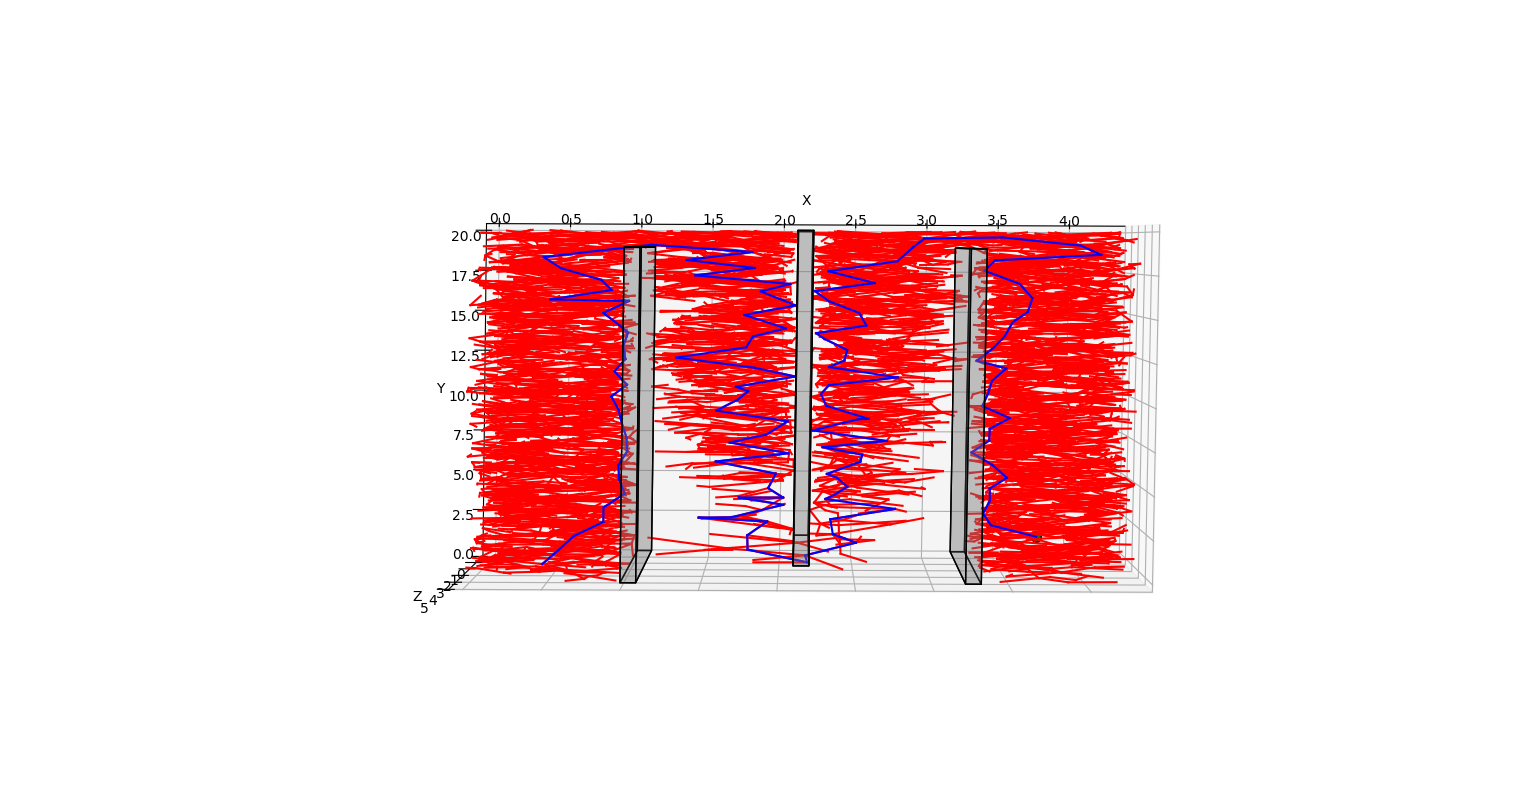
\includegraphics[width=0.7\textwidth]{./images/RRT-monza.png}
    \caption{RRT-monza}
    \label{RRT-monza}
\end{figure}

\begin{figure}[H]
	\centering
    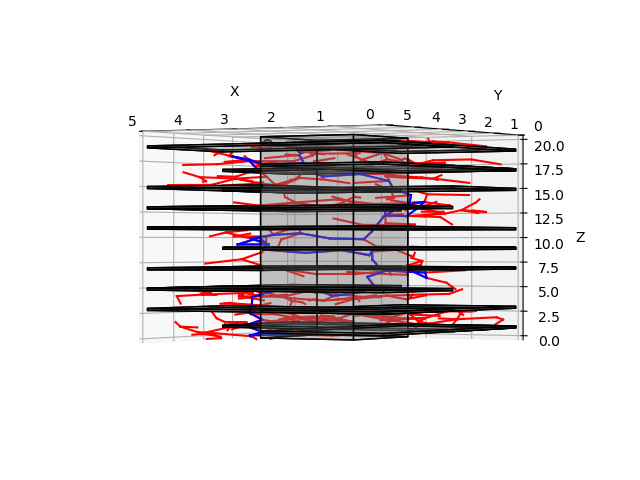
\includegraphics[width=0.7\textwidth]{./images/RRT-tower.png}
    \caption{RRT-tower}
    \label{RRT-tower}
\end{figure}

The collision detection is inspired by the ray-box intersection algorithm\cite{raybox}.

\begin{thebibliography}{999}

    \bibitem{raybox}
    Williams, Amy, et al. "An efficient and robust ray-box intersection algorithm." Journal of graphics tools 10.1 (2005): 49-54.

    \bibitem{RTAA}
    Koenig, Sven, and Maxim Likhachev. "Real-time adaptive A." Proceedings of the fifth international joint conference on Autonomous agents and multiagent systems. ACM, 2006.
    
\end{thebibliography}
    
\end{document}